\documentclass[10pt,twocolumn]{article}

\usepackage[margin=0.72in]{geometry}
\usepackage[T1]{fontenc}
\usepackage[utf8]{inputenc}
\usepackage{lmodern}
\usepackage{microtype}
\usepackage{amsmath,amssymb}
\usepackage{booktabs}
\usepackage{graphicx}
\usepackage{xcolor}
\usepackage{url}
\usepackage[hidelinks]{hyperref}
\usepackage{enumitem}
\usepackage{caption}
\usepackage{subcaption}

\newcommand{\method}{GSN-QAOA}
\newcommand{\E}{\mathbb{E}}
\newcommand{\Prob}{\mathbb{P}}
\newcommand{\todoauthor}{Anonymous Authors}

\title{Graph-Scale Normalization Enables Zero-Shot Transfer of\\Evolutionary QAOA Schedules for Maximum Independent Set}
\author{\todoauthor\\\small Author names and affiliations withheld for review}
\date{}

\begin{document}
\maketitle

\begin{abstract}
Variational parameter transfer can amortize the classical optimization cost of the Quantum Approximate Optimization Algorithm (QAOA), but parameters learned on one constrained graph often fail when the Ising coefficient scale changes with graph degree and penalty strength. We study a deliberately lightweight alternative to graph-conditioned neural transfer: divide each Maximum Independent Set (MIS) Ising Hamiltonian by its largest-magnitude local coefficient, then evolve one shared depth-two schedule across a small graph family. The schedule has only five parameters, requires no graph encoder and is applied to every target without parameter refinement. Twelve paired optimization replicates were evaluated by exact statevector simulation on 15 frozen QOBLIB-derived graphs spanning 17--24 qubits. Across four held-out suites, normalized differential evolution improved the raw composite score over the identical unnormalized protocol by $0.0599$--$0.1081$; every paired bootstrap 95\% interval excluded zero and every paired $t$-test gave $p\leq0.0102$. On the final predeclared confirmatory suite the improvement was $0.0691$ (95\% bootstrap CI $[0.0344,0.1055]$, $p=0.00374$, 10/12 wins). A second suite of six predeclared random induced subgraphs produced $0.1081$ ($[0.0579,0.1603]$, $p=0.00231$), while unconditional approximation ratio and feasible probability improved independently of the composite score. Equal-budget differential evolution was better than normalized random search on average but not reliably on held-out graphs, so the evidence supports normalization rather than optimizer superiority. Routing audits show that dense 24-qubit instances can expand from 600 logical two-qubit operations to 2,943--10,836 routed operations, precluding a hardware-performance claim. These results identify coefficient normalization as a low-cost, reproducible control for cross-graph QAOA transfer and sharply delimit what it does not solve.
\end{abstract}

\section{Introduction}

QAOA alternates a problem Hamiltonian and a mixer, with angles chosen by a classical optimization loop \cite{farhi2014qaoa}. Even at low depth, this loop can dominate the number of quantum evaluations. Reusing parameters across related problems is therefore attractive: optimize once, then deploy many times. Existing transfer work has identified parameter concentration and graph-structural donor selection for MaxCut \cite{galda2023similarity,falla2024graph}, while recent MIS studies use graph attention networks to select donor parameters \cite{xu2025gat}. Graph-conditioned meta-optimizers go further by generating instance-aware optimization trajectories \cite{nguyen2026meta}. These methods trade target optimization for a learned representation, labels, target embeddings, or a larger training corpus.

This paper asks a narrower question. Before learning which graph should donate parameters, can one remove a simple source of graph dependence from the Hamiltonian itself? In the standard MIS QUBO, the magnitude of a local Ising field grows with vertex degree and the penalty coefficient. A fixed QAOA angle therefore represents a different physical rotation on two graphs with different maximum degrees. We normalize the Ising Hamiltonian by its largest local coefficient and train one shared schedule. The target graph changes only the normalized operator, not the five-dimensional genome.

The contribution is empirical and intentionally modest:

\begin{enumerate}[leftmargin=*,nosep]
    \item We formulate graph-scale normalization for penalty-based MIS QAOA and combine it with a shared multi-instance evolutionary objective.
    \item We use paired optimization seeds, equal budgets, exact enumeration, exact statevectors, frozen graph suites, and raw feasibility-aware metrics to isolate normalization from the optimizer.
    \item We confirm the effect on 15 held-out QOBLIB-derived graphs, including six random induced subgraphs fixed before evaluation to rule out a \emph{first-$k$} vertex-order artifact.
    \item We report negative controls: the robust mean/min objective is not significantly better than simpler training objectives; a feasibility-preserving mixer collapses to an embedded greedy construction; and hardware routing overhead remains prohibitive.
\end{enumerate}

We do not claim quantum advantage, superiority to classical MIS solvers, or a general parameter-transfer theorem. The claim supported here is that maximum-coefficient normalization materially improves the zero-shot transfer of one low-depth penalty-QAOA policy under the tested protocol.

\section{Related work}

\paragraph{QAOA parameter transfer.}
Parameter concentration motivates transferring angles from small donor graphs to larger acceptors. Similarity-based and representation-learning approaches relate successful MaxCut transfer to local structures and degree properties \cite{galda2023similarity,falla2024graph}. Xu \emph{et al.} train on 12- and 14-vertex graphs and use a graph attention network (GAT) for MIS donor selection, integrating the result into a decomposition workflow \cite{xu2025gat}. Nguyen and Safro condition a parameter-generating meta-optimizer on graph embeddings across several problem classes \cite{nguyen2026meta}. In contrast, \method{} has no target-conditioned component: every target receives the same schedule, and normalization is computed directly from Hamiltonian coefficients.

\paragraph{Evolutionary variational optimization.}
Differential evolution (DE) is a derivative-free population method designed for nonconvex continuous spaces \cite{storn1997differential}. Evolution is not itself our novelty. We use DE because it gives a transparent, fixed evaluation budget and naturally optimizes a worst-case-aware objective. Equal-budget uniform random search controls whether any gain should be attributed to evolution.

\paragraph{Constraint handling.}
Penalty Hamiltonians expose infeasible bit strings but are circuit-simple. Alternating-operator constructions and subspace mixers can preserve feasibility \cite{hadfield2019alternating,fuchs2024lx}. Newer constrained hypercube and warm-start XY approaches continue this line \cite{wang2026hypercube,aqarios2026warmstart}. We tested a feasibility-preserving MIS construction as a negative control, but its strongest schedule implements a classical degree-ordered greedy choice inside a unitary. We therefore exclude it from the primary novelty claim.

\paragraph{Benchmarking.}
QOBLIB provides curated optimization instances and validation infrastructure \cite{koch2026qoblib}. Metriq-Gym provides reviewable, cross-provider quantum benchmark implementations \cite{metriqgym}. Our main MIS study uses QOBLIB instances. Separately, we execute Metriq-Gym's actual linear-ramp QAOA circuit locally as an integration cross-check; it is not evidence for the MIS hypothesis.

\section{Method}

\subsection{MIS penalty Hamiltonian}

For a graph $G=(V,E)$ and binary variables $x_i\in\{0,1\}$, we minimize
\begin{equation}
 C_G(x;\lambda)=-\sum_{i\in V}x_i+\lambda\sum_{(i,j)\in E}x_ix_j,
 \label{eq:qubo}
\end{equation}
where $\lambda>1$ penalizes adjacent selected vertices. With $x_i=(1-Z_i)/2$ and irrelevant constants removed,
\begin{equation}
 H_C(G,\lambda)=\sum_i h_i Z_i+\sum_{(i,j)\in E}JZ_iZ_j,
\end{equation}
where
\begin{equation}
 h_i=\frac{1}{2}-\frac{\lambda d_i}{4},\qquad J=\frac{\lambda}{4}.
 \label{eq:coefficients}
\end{equation}
Here $d_i$ is the degree of vertex $i$. Thus, even for fixed $\lambda$, the largest rotation generator grows with graph degree.

\subsection{Graph-scale normalization}

We define
\begin{equation}
 s(G,\lambda)=\max\left(\max_i |h_i|,|J|,10^{-12}\right),
 \qquad \widetilde H_C=H_C/s.
 \label{eq:normalization}
\end{equation}
This is not an instance-specific angle optimization: $s$ is an algebraic property of the deployed Hamiltonian. It makes the maximum magnitude of any local $Z$ or $ZZ$ coefficient equal to one. The unnormalized control uses the identical circuit, genome, optimizer and budget, but sets $s=1$.

At depth $p=2$, the state is
\begin{equation}
 |\psi_G(\theta)\rangle=\prod_{\ell=1}^{2}
 e^{-i\beta_\ell H_M}e^{-i\gamma_\ell\widetilde H_C(G,\lambda)}|+\rangle^{\otimes |V|},
\end{equation}
with $H_M=\sum_i X_i$ and shared genome
$\theta=(\lambda,\beta_1,\beta_2,\gamma_1,\gamma_2)$. Bounds are $\lambda\in[1.05,4]$, $\beta_\ell\in[0,\pi]$, and $\gamma_\ell\in[0,2\pi]$.

\subsection{Training objective}

Let $F_G$ be the feasible independent sets and $\alpha(G)$ the exact MIS size. For the exact output distribution $P_\theta(x|G)$, our raw score is
\begin{equation}
 \begin{aligned}
 S_G(\theta)={}&
 \frac{\E[|x|\mathbf{1}\{x\in F_G\}]}{\alpha(G)}\\
 &+0.25\Prob(x\in \operatorname{MIS}(G))
 +0.10\Prob(x\in F_G).
 \end{aligned}
 \label{eq:score}
\end{equation}
The first term is an unconditional feasible approximation ratio: infeasible mass contributes zero rather than being repaired. We train across four graphs using
\begin{equation}
 S_{\mathrm{train}}=0.7\,\operatorname{mean}_G S_G+0.3\,\min_G S_G.
 \label{eq:aggregate}
\end{equation}
Because Eq.~\eqref{eq:score} is custom, all conclusions are also audited on its constituent raw metrics. An objective ablation compares Eq.~\eqref{eq:aggregate} with mean-only and single-instance DE.

\section{Experimental protocol}

\subsection{Optimization and pairing}

We run 12 independent replicates. Each method receives exactly 300 objective evaluations per replicate. DE uses a population of 15; random search draws 300 independent genomes. For the normalization comparison, normalized and unnormalized DE share the same replicate seed. The inferential unit is the replicate-level score averaged over a frozen graph suite, not an individual bit string or graph.

We report paired mean differences, nonparametric paired bootstrap 95\% intervals, two-sided paired $t$-tests, one-sided Wilcoxon signed-rank tests, and win counts. Promotion required four conditions fixed before evaluation: positive mean, a strictly positive bootstrap interval, paired $t$-test $p<0.05$, and a majority of replicate wins. Suites reuse the same 12 trained schedules, so suite-level tests are corroborating views and are not combined as independent evidence.

\subsection{Graphs and split discipline}

Training uses the 17-vertex QOBLIB \texttt{mammalia-kangaroo-interactions} instance and three fixed induced subgraphs of 11, 13 and 15 vertices. A separate 17-vertex graph is used for validation. We then evaluate four held-out suites:

\begin{itemize}[leftmargin=*,nosep]
    \item three frozen 17-qubit graphs from \texttt{karate}, \texttt{chesapeake}, and \texttt{aves-sparrow-social};
    \item a 20/22/24-qubit scale-up suite from \texttt{ibm32}, \texttt{football}, and \texttt{johnson8-2-4};
    \item a final confirmatory 20/22/24-qubit suite from \texttt{insecta-ant-colony1-day38}, \texttt{sloane\_1dc\_64}, and \texttt{hamming6-4};
    \item six random induced subgraphs: two each from sparse \texttt{es60fst01} ($n=20$), medium-density \texttt{aves-sparrow-social} ($n=22$), and dense \texttt{MANN-a9} ($n=24$).
\end{itemize}

The random subsets, seeds, and exact vertex lists were written to the artifact's novelty audit before schedule evaluation. Across the last three suites, graph densities range from 0.026 to 0.927 and exact optima range from 2 to 16. Exact enumeration is limited to 24 vertices by design.

\subsection{Simulation and controls}

Exact statevectors are computed with Qiskit Aer \cite{qiskit2024}. No sampling noise enters the primary endpoints. Finite-shot sampling is derived from frozen exact distributions for ancillary checks. The controls are:

\begin{description}[leftmargin=*,style=nextline,nosep]
    \item[Unnormalized DE.] Same QUBO, genome, seeds and 300-evaluation DE protocol, without Eq.~\eqref{eq:normalization}.
    \item[Normalized random.] Same normalized objective and 300-evaluation budget, replacing DE by uniform random search.
    \item[Uniform state.] Analytical $|+\rangle^{\otimes n}$ baseline for feasibility and unconditional ratio.
    \item[Classical sanity.] Minimum-degree greedy and 1,000 random-order greedy restarts, explicitly not runtime matched, to prevent a quantum-advantage interpretation.
\end{description}

\section{Results}

\subsection{Normalization transfers across every frozen suite}

Table~\ref{tab:primary} and Fig.~\ref{fig:forest} show the main result. The paired score difference is positive in all four suites, every bootstrap interval excludes zero, and all paired $t$-tests pass the predeclared 0.05 threshold. On the final confirmatory suite, normalized DE raises the mean score from 0.1332 to 0.2023, a difference of 0.0691. The independently declared random-subset suite gives the largest effect, 0.1081, despite spanning extremely sparse to extremely dense subgraphs. This argues against a source-file vertex-order artifact.

\begin{table*}[t]
\centering
\caption{Paired normalization effect on frozen suites. Means are over 12 independently optimized schedules after averaging each schedule over the suite. CIs are paired bootstrap intervals.}
\label{tab:primary}
\small
\begin{tabular}{lrrrrrr}
\toprule
Suite & Normalized & Unnormalized & Difference & 95\% CI & $p_t$ & Wins \\
\midrule
Frozen 17-qubit & 0.2509 & 0.1676 & 0.0833 & [0.0465, 0.1247] & 0.00218 & 11/12 \\
Scale-up 20--24 & 0.2025 & 0.1426 & 0.0599 & [0.0254, 0.0987] & 0.01015 & 10/12 \\
Confirmatory 20--24 & 0.2023 & 0.1332 & 0.0691 & [0.0344, 0.1055] & 0.00374 & 10/12 \\
Random subsets 20--24 & 0.2455 & 0.1374 & 0.1081 & [0.0579, 0.1603] & 0.00231 & 10/12 \\
\bottomrule
\end{tabular}
\end{table*}

\begin{figure}[t]
\centering
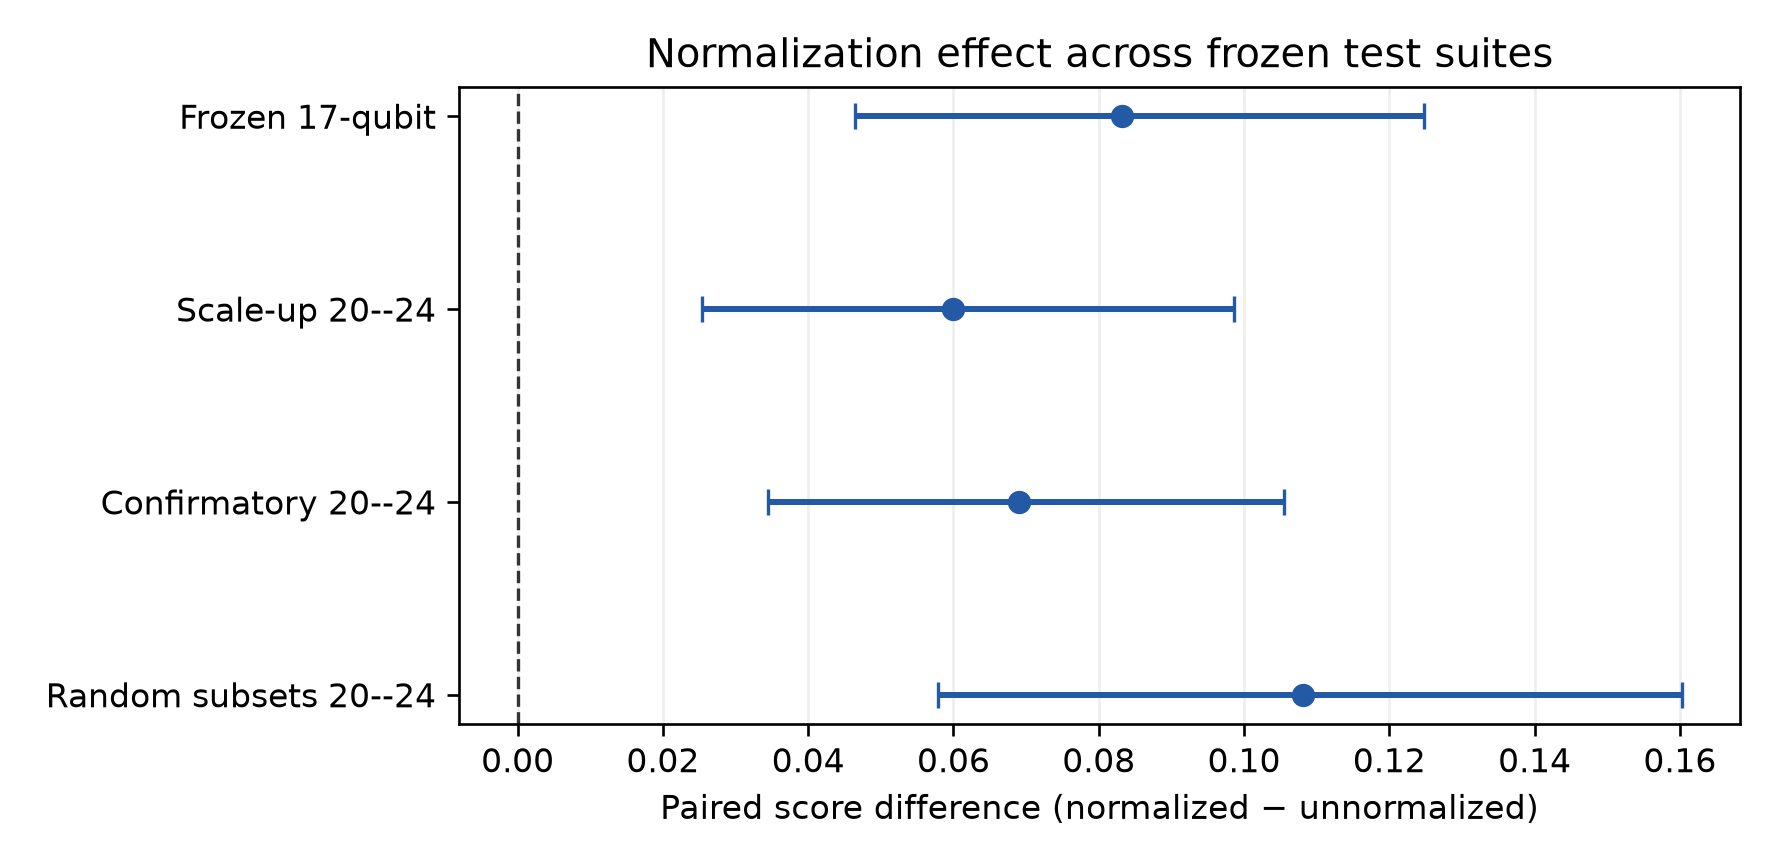
\includegraphics[width=\columnwidth]{figures/normalization_forest.png}
\caption{Mean paired score improvements and 95\% paired bootstrap intervals. The dashed line denotes no effect. The same schedules are evaluated in every suite, so the rows are not statistically independent.}
\label{fig:forest}
\end{figure}

\subsection{The effect is not created by the composite score}

On the final confirmatory suite, normalization improves unconditional approximation ratio by 0.0544 (95\% CI $[0.0283,0.0821]$, $p=0.00297$) and feasible probability by 0.1466 ($[0.0432,0.2479]$, $p=0.0215$). Optimum probability changes by only $4.97\times10^{-5}$ and is not significant ($p=0.601$).

The random-subset suite is consistent: unconditional approximation ratio improves by 0.0888 ($[0.0467,0.1318]$, $p=0.00238$), and feasible probability by 0.1648 ($[0.0496,0.2792]$, $p=0.0213$). Optimum probability increases by 0.0113 with a positive bootstrap interval, but the paired $t$-test is marginal ($p=0.0557$) because the replicate distribution is skewed. The normalization effect is therefore best described as moving probability mass toward larger feasible solutions, not reliably concentrating it on the exact optimum.

\begin{figure}[t]
\centering
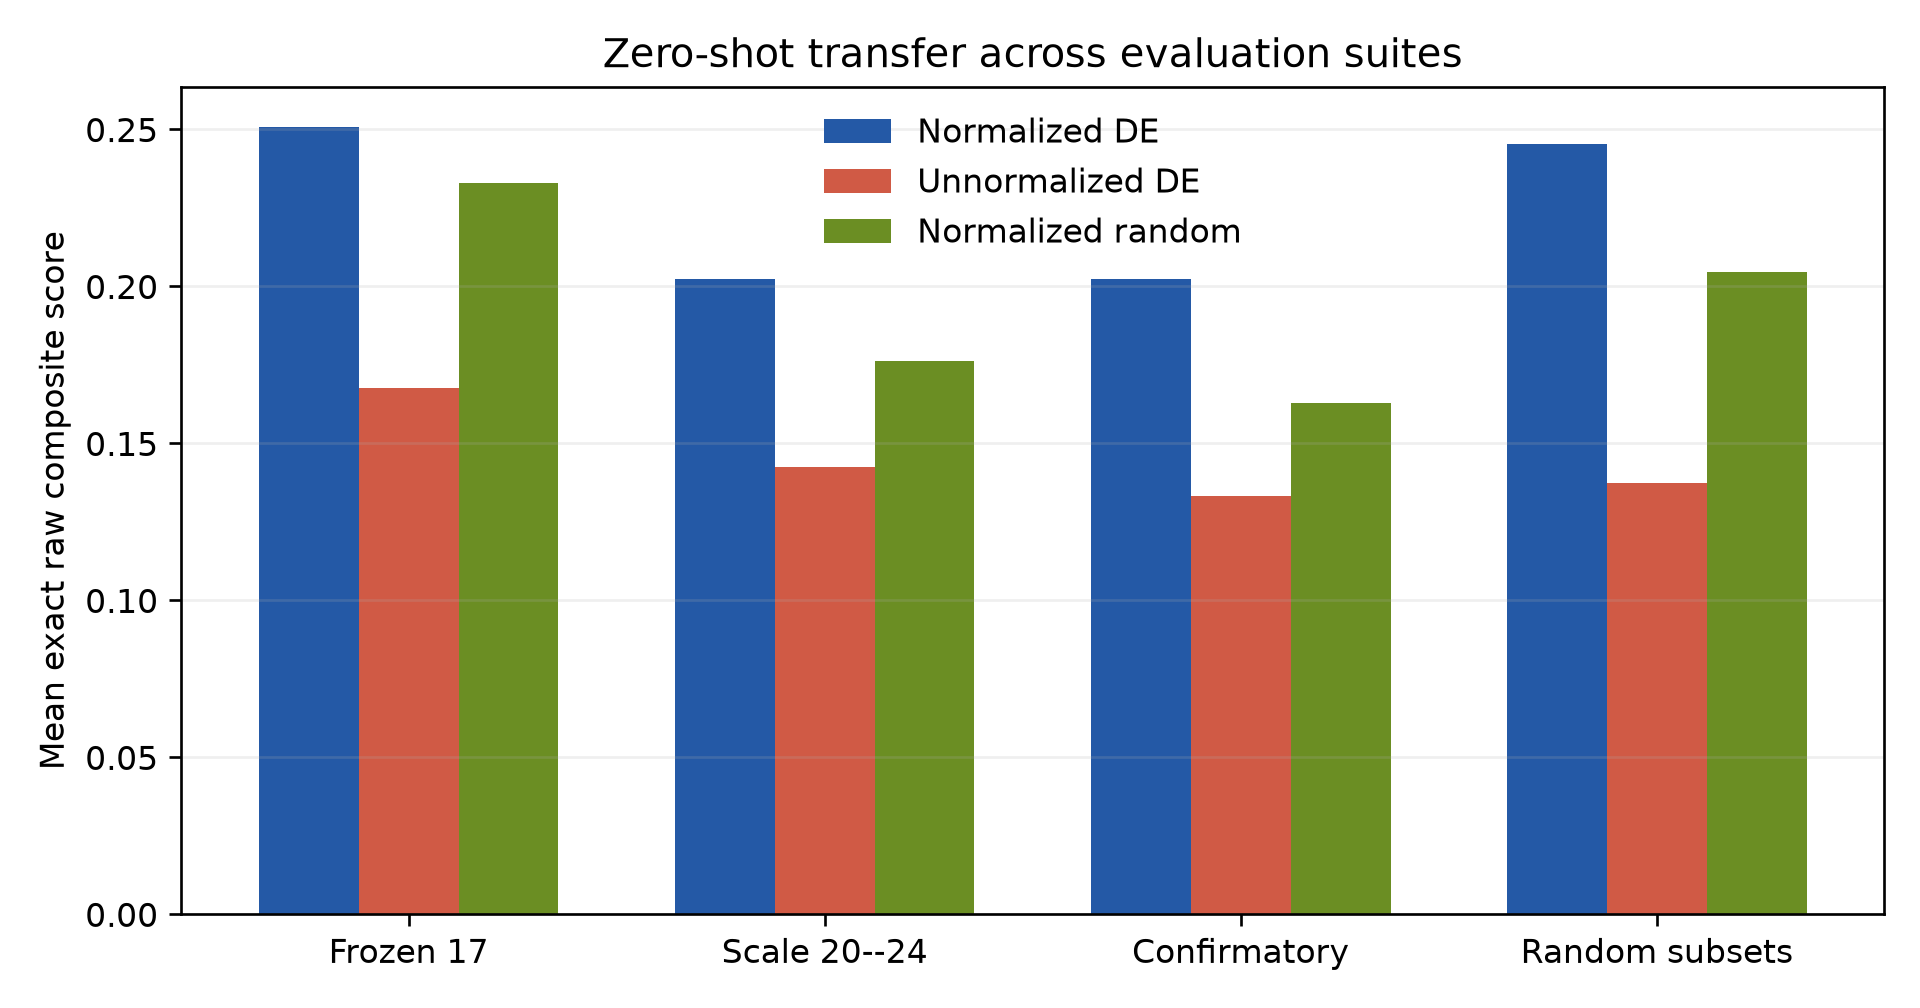
\includegraphics[width=\columnwidth]{figures/suite_method_means.png}
\caption{Mean exact raw scores. Normalized DE is consistently above unnormalized DE. Its advantage over equal-budget normalized random search is smaller and not statistically reliable on held-out suites.}
\label{fig:means}
\end{figure}

\subsection{Evolution is secondary, not the supported novelty}

DE beats normalized random search on the training objective by 0.0649 ($p=0.0242$, 10/12 wins). Held-out differences remain positive but are not conventionally significant: 0.0181 on frozen 17-qubit graphs ($p=0.452$), 0.0262 at 20--24 qubits ($p=0.226$), 0.0393 on the confirmatory suite ($p=0.0614$), and 0.0408 on random subsets ($p=0.358$). We therefore reject a strong claim that evolution itself improves transfer. It supplies a reproducible policy ensemble; normalization supplies the robust effect.

Likewise, the robust mean/min training objective does not significantly outperform mean-only DE or single-instance DE on frozen targets. Against mean-only training the difference is 0.0215 ($p=0.392$); against single-instance training it is 0.0068 ($p=0.753$). These negative ablations narrow the contribution further.

\subsection{Classical sanity check}

Across 12 scale-up, confirmatory and random-subset graphs, minimum-degree greedy reaches the exact optimum on 8 graphs and has mean approximation ratio 0.899. The best of 1,000 random-order greedy restarts reaches the exact optimum on all 12. These heuristics are not runtime matched, but they make the interpretation unambiguous: the present result concerns QAOA parameter transfer and experimental methodology, not competitive MIS solution quality or quantum advantage.

\section{Hardware and benchmark audits}

\subsection{Routing cost dominates at density}

We transpile the champion depth-two circuit to a line, a $5\times5$ grid, and a 30-node hexagonal lattice. Optimization level zero with deterministic basic routing is used as a reproducible upper-bound audit; attempts to perform large SABRE searches were impractical locally. Table~\ref{tab:routing} shows that routing overhead grows sharply with density. The 24-qubit Johnson subgraph contains 600 logical two-qubit operations, but basic routing produces 2,943 on a grid, 3,657 on a hexagonal lattice and 10,836 on a line.

\begin{table}[t]
\centering
\caption{Two-qubit operation counts after routing.}
\label{tab:routing}
\small
\begin{tabular}{lrrrr}
\toprule
Graph & Logical & Line & Grid & Hex \\
\midrule
20q IBM & 172 & 1,822 & 613 & 787 \\
22q football & 208 & 2,842 & 892 & 1,114 \\
24q Johnson & 600 & 10,836 & 2,943 & 3,657 \\
\bottomrule
\end{tabular}
\end{table}

\begin{figure}[t]
\centering
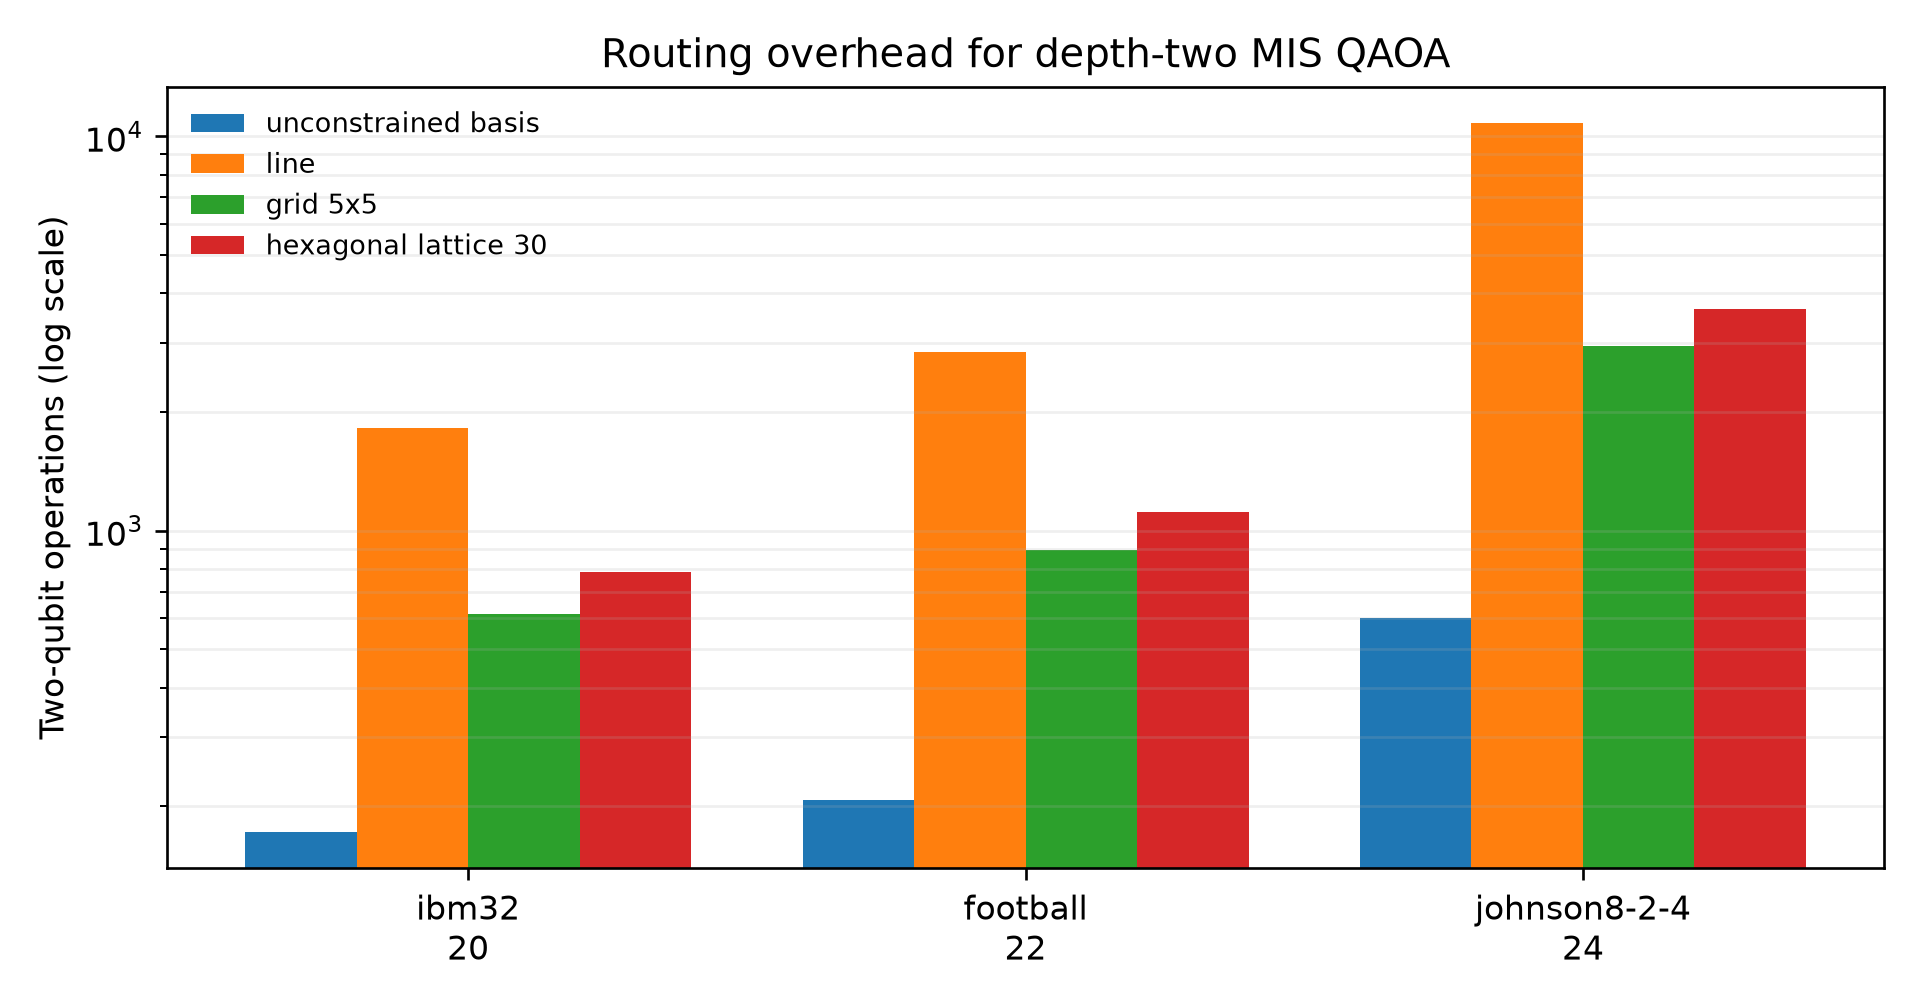
\includegraphics[width=\columnwidth]{figures/routing_overhead.png}
\caption{Routing resource audit. The logarithmic axis exposes the order-of-magnitude increase on restricted connectivity.}
\label{fig:routing}
\end{figure}

An independent-error proxy using 0.1\% one-qubit, 1\% two-qubit and 2\% readout error gives no-error survival $4.54\times10^{-14}$ for the 24-qubit grid circuit. This proxy is not a noise simulation. Routed noisy matrix-product-state simulation was attempted at 128 and then 16 shots but did not finish the first 20-qubit graph within a practical CPU budget. We report the failure rather than extrapolating a hardware result.

\subsection{Metriq-Gym cross-check}

As an integration check independent of our MIS implementation, we invoke \texttt{metriq\_gym.circuits.qaoa\_circuit} directly on a 10-qubit weighted one-dimensional MaxCut instance with 4,096 Aer shots. Linear-ramp QAOA improves from approximation ratio 0.6735 at $p=3$ to 0.7523 at $p=10$, while optimum probability rises from 0.0093 to 0.0251. The uniform exact ratio is 0.5. This verifies that the local environment executes an external benchmark implementation, but it tests neither MIS nor our normalization hypothesis.

\begin{figure}[t]
\centering
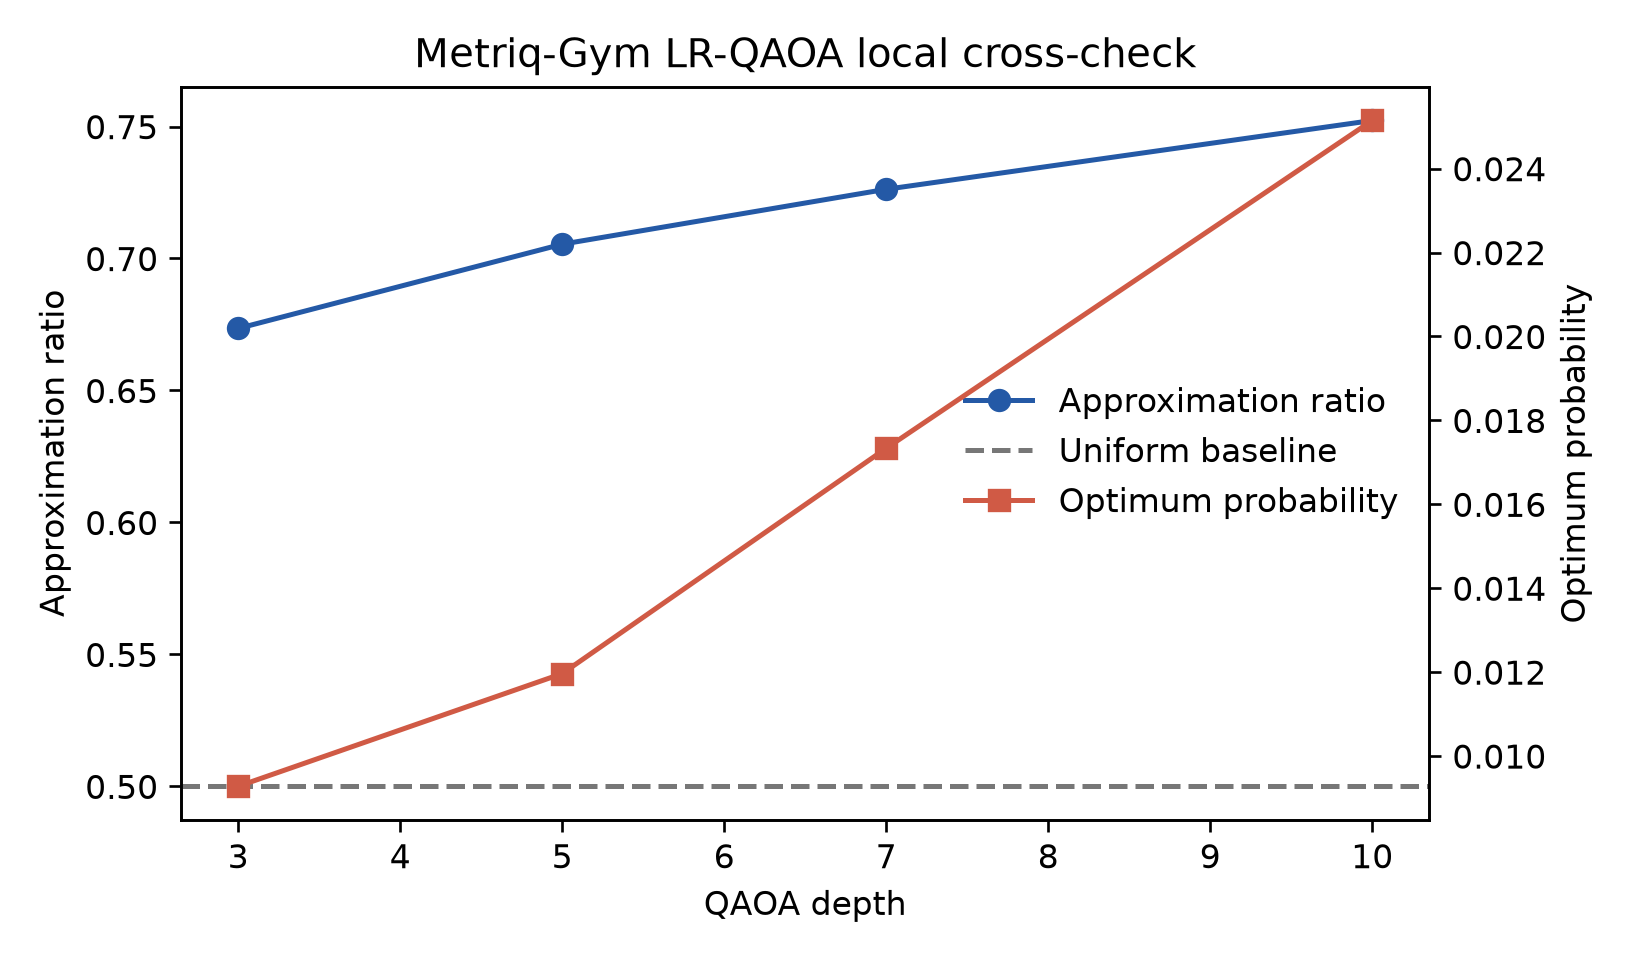
\includegraphics[width=\columnwidth]{figures/metriq_crosscheck.png}
\caption{Local Metriq-Gym LR-QAOA cross-check.}
\label{fig:metriq}
\end{figure}

\section{External baseline reproducibility}

We audited the public repository accompanying the closest learned MIS transfer baseline \cite{xu2025gat} at commit \texttt{ab8434f}. It includes an Apache-2.0 checkpoint and cluster/parameter tables. However, its checked-in large-graph script requires an absent \texttt{mis\_output\_2p} directory and missing 24-node train/test Graph2Vec files at the declared paths. The released evaluation is also structurally different: ER donors and acceptors, target Node2Vec features, GAT cluster selection, a fixed 1.5 penalty, and one donor schedule rather than a graph-independent policy. Consequently, inserting a number from a partially reconstructed pipeline would not be an apples-to-apples baseline. We cite it as the closest methodological comparator and provide a line-level artifact audit. The contemporaneous graph-conditioned meta-optimizer \cite{nguyen2026meta} had no public implementation or checkpoint located at audit time.

This limitation does not turn normalized random search into a state-of-the-art comparator. Rather, it defines the evidence precisely: our paired ablation isolates whether normalization helps within one reproducible protocol. A future benchmark should standardize the Hamiltonian convention, depth, target graphs, supervision budget, and whether target embeddings count as adaptation before comparing learned and graph-independent transfer.

\section{Discussion}

Why does Eq.~\eqref{eq:normalization} help? Without normalization, a common $\gamma$ induces rotations proportional to $\lambda d_i$; a dense target can move far outside the phase scale experienced during training. Maximum-coefficient normalization bounds every local phase generator and preserves the relative pattern of fields and couplings. It therefore removes a global scale nuisance while retaining graph structure. The result is compatible with, rather than opposed to, learned transfer: a graph-conditioned predictor could generate angles for normalized Hamiltonians.

The effect is strongest on random induced subgraphs, including nearly empty and nearly complete cases. This does not prove distribution-free robustness. Sparse subgraphs have many isolated vertices, and dense subgraphs can have very small MIS optima; both may be easier than intermediate structured cases. More importantly, all training graphs derive from one source instance. The broad source diversity lies in evaluation, not training.

The feasible-mixer negative control illustrates another interpretive hazard. Its best evolved schedule prepared the degree-ordered greedy independent set with almost unit probability. Feasibility and even optimality on a small suite were real, but the mechanism was a classical greedy algorithm encoded by sequential controlled rotations. Treating that result as a quantum improvement would overstate the contribution. We retain it in the artifact as a diagnostic and exclude it from the proposed method.

\section{Limitations}

\begin{itemize}[leftmargin=*]
    \item The maximum size is 24 qubits, imposed by exact enumeration and statevector validation. No asymptotic claim follows.
    \item Training diversity is limited to induced subgraphs of one 17-vertex source. The study demonstrates extrapolation across held-out sources, not universal training.
    \item The score in Eq.~\eqref{eq:score} is application-specific. Raw-metric sensitivity supports feasibility and unconditional ratio, but not consistent exact-optimum concentration.
    \item Statistical replicates are optimizer seeds, not new training families. Reusing schedules across suites makes the four rows in Table~\ref{tab:primary} dependent.
    \item No named QPU result is reported. Routing counts use synthetic coupling maps and an analytical independent-error proxy.
    \item The strongest learned baselines could not be reproduced comparably from their released artifacts, so the work is an ablation study rather than a leaderboard result.
    \item Simple classical greedy restarts solve every audited graph, ruling out a practical or quantum-advantage claim.
\end{itemize}

\section{Reproducibility statement}

The artifact contains all code, frozen graph declarations, raw JSON, checkpoints, figures, tests, and a SHA-256 manifest. The primary experiment uses Python 3.13, Qiskit 2.5.1, Qiskit Aer 0.17.2, NumPy 2.5.1, SciPy 1.18.0 and Matplotlib 3.11.1 on Windows 11. A PowerShell driver reruns the research cycle. Six unit tests verify graph parsing, exact MIS enumeration, normalized circuits, metrics, deterministic search, and repair. Exact vertex lists for all induced graphs are embedded in result metadata. The external GAT repository is preserved separately and is not included in our artifact hash manifest.

\section{Conclusion}

Dividing an MIS Ising Hamiltonian by its maximum local coefficient is a small intervention, but it consistently improves the zero-shot transfer of shared depth-two QAOA schedules across the tested graph sizes, densities, sources, and vertex-selection rules. The strongest evidence is not a single champion: it is the agreement of 12 paired optimization replicates, frozen-suite confidence intervals, raw-metric sensitivity, and a second predeclared random-subgraph audit. Equally important, the experiments reject broader narratives: DE is not reliably superior to equal-budget random search on held-out graphs, the robust objective is not established as better, a feasible mixer can hide classical greedy computation, and normalization does not address routing noise. This combination of a positive narrow result and explicit negative controls makes graph-scale normalization a useful default for future parameter-transfer studies and a clean preprocessing step for more expressive learned methods.

\bibliographystyle{plain}
\bibliography{references}

\clearpage
\onecolumn
\appendix
\section{Supplementary numerical results}

\begin{table}[h]
\centering
\caption{Raw-metric normalization sensitivity on the two predeclared 20--24-qubit suites.}
\small
\begin{tabular}{llrrrr}
\toprule
Suite & Metric & Difference & 95\% CI & $p_t$ & Wins \\
\midrule
Confirmatory & Composite score & 0.06908 & [0.03443, 0.10552] & 0.00374 & 10/12 \\
Confirmatory & Unconditional ratio & 0.05441 & [0.02826, 0.08215] & 0.00297 & 10/12 \\
Confirmatory & Feasible probability & 0.14656 & [0.04315, 0.24793] & 0.02147 & 9/12 \\
Confirmatory & Optimum probability & 0.000050 & [$-0.000114$, 0.000231] & 0.60148 & 9/12 \\
Random subsets & Composite score & 0.10807 & [0.05787, 0.16027] & 0.00231 & 10/12 \\
Random subsets & Unconditional ratio & 0.08877 & [0.04672, 0.13177] & 0.00238 & 10/12 \\
Random subsets & Feasible probability & 0.16485 & [0.04964, 0.27924] & 0.02127 & 8/12 \\
Random subsets & Optimum probability & 0.01126 & [0.00441, 0.02234] & 0.05571 & 11/12 \\
\bottomrule
\end{tabular}
\end{table}

\section{Artifact map}

The machine-readable sources for every value in the paper are:
\begin{itemize}[leftmargin=*]
    \item \texttt{results\_multitask\_normalized/results.json}: schedules, training, validation and frozen 17-qubit tests;
    \item \texttt{results\_scaleup\_20\_24/results.json}: first scale-up suite;
    \item \texttt{results\_confirmatory/results.json}: final confirmatory suite;
    \item \texttt{results\_random\_subsets/results.json}: random-induced-subgraph audit;
    \item \texttt{results\_objective\_ablation/results.json}: mean/min objective ablation;
    \item \texttt{results\_feasible\_mixer/results.json}: feasibility-preserving negative control;
    \item \texttt{results\_hardware\_audit/results.json}: routing and error proxy;
    \item \texttt{results\_classical\_sanity/results.json}: uniform and greedy controls;
    \item \texttt{results\_metriq\_lrqaoa/result.json}: Metriq-Gym cross-check.
\end{itemize}

\end{document}
